\documentclass[letterpaper]{article}

\usepackage[left=0.8in,top=0.8in,right=0.8in,bottom=0.8in]{geometry} % margins

\usepackage{lmodern}
\usepackage[T1]{fontenc}
\usepackage{pxfonts}

\usepackage{graphics}
\usepackage{tikz}
\usetikzlibrary{shadows,arrows,shapes,decorations.pathmorphing,backgrounds,positioning,fit,petri,matrix,graphs}
\usetikzlibrary{calc}

\definecolor{darkgray}{rgb}{0.4,0.4,0.4}
\definecolor{gblue1}{rgb}{1.0,0.6,0.6}
\definecolor{blue2}{rgb}{0.5,0.7,1.0}
\definecolor{lightgreen}{rgb}{0.9,1.0,0.9}
\definecolor{lightblue}{rgb}{0.9,0.9,1.0}
\definecolor{turquoise}{rgb}{0.3,0.9,0.8}
\definecolor{aquamarine}{rgb}{0.5,1.0,0.8}
\definecolor{orchid}{rgb}{0.8,0.6,0.7}
\definecolor{darkorangered}{rgb}{0.95,0.3,0.1}
\definecolor{darkred}{rgb}{0.95,0.0,0.0}
\definecolor{orange}{rgb}{0.9,0.6,0.3}


\tikzset{
  %%basic/.style  = {draw, text width=2cm, drop shadow, font=\sffamily, rectangle},
  basic/.style  = {draw, text width=2cm, drop shadow, rectangle},
  root/.style   = {basic, rounded corners=2pt, thin, align=center, fill=green!30},
  box-round-1/.style = {basic, rounded corners=4pt, thin, align=center, fill=lightblue, text width=12em, text height=1em},
  box-round-2/.style = {basic, rounded corners=4pt, thin, align=center, fill=lightgreen, text width=12em, text height=1em},
  box-round-3/.style = {basic, rounded corners=4pt, thin, align=center, fill=turquoise!40, text width=9em, text height=0.8em},
  box-round-4/.style = {basic, rounded corners=4pt, thin, align=center, fill=blue!16, minimum size=2.2cm},
  bend angle=45,
  in-arrow/.style={<-,shorten <=1pt,>=stealth',thick},
  out-arrow/.style={->,shorten >=1pt,>=stealth',thick}
}

\pgfdeclareimage[interpolate=true,width=1.2cm,height=1.2cm]{image-electrum}{/home/tarok/Finance/Bitcoin/Electrum/electrum.png}


\begin{document}

\pagestyle{empty}

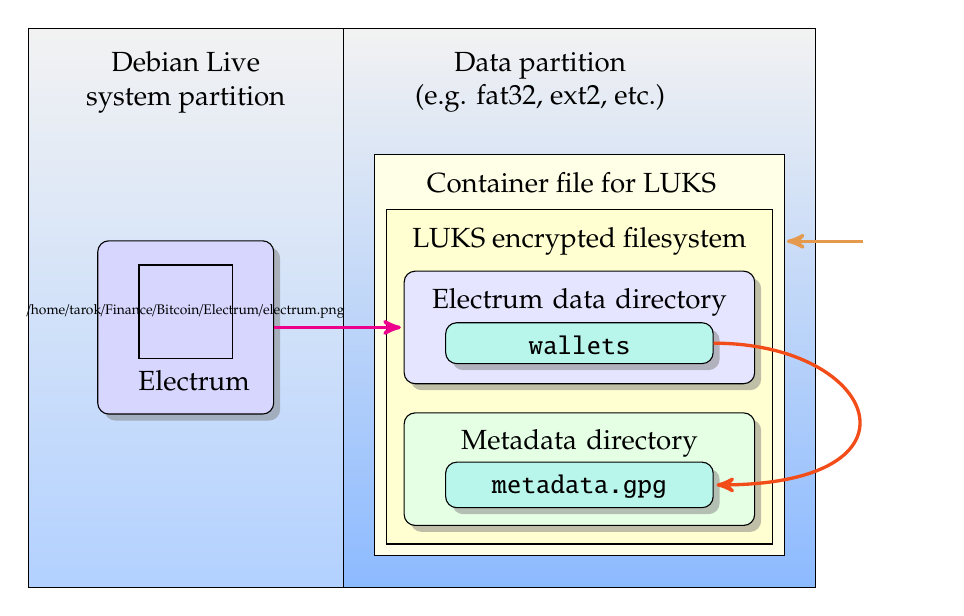
\begin{tikzpicture}

  \draw[top color=gray!10!, bottom color=blue2!60!] (0.0,0.0) rectangle (4.0,7.1);
  \draw[top color=gray!10!, bottom color=blue2!90!] (4.0,0.0) rectangle (10.0,7.1);

  \draw (2.0,7.1) node[below=5pt,align=center] {Debian Live\\ system partition};
  \draw (6.5,7.1) node[below=5pt,align=center] {Data partition\\ (e.g. fat32, ext2, etc.)};

  \draw[top color=yellow!09!, bottom color=yellow!09!]  (4.4,0.4) rectangle (9.6,5.5);
  \draw[top color=yellow!18!, bottom color=yellow!18!]  (4.55,0.55) rectangle (9.45,4.8);
  \draw (6.9,5.5) node[below=3pt,align=center] (container) {Container file for LUKS};
  \draw (7.0,4.8) node[below=3pt,align=center] (luks-title) {LUKS encrypted filesystem};

  \draw (7.0,3.3) node[box-round-1,align=center] (data-dir) {Electrum data directory\\ \hspace{1em}\\ \hspace{1em}};
  \draw (7.0,3.1) node[box-round-3,align=center] (wallets) {\texttt{wallets}};
  \draw (7.0,1.5) node[box-round-2,align=center] (metadata-dir) {Metadata directory\\ \hspace{1em}\\ \hspace{1em}};
  \draw (7.0,1.3) node[box-round-3,align=center] (metadata) {\texttt{metadata.gpg}};

  \draw (2.0,3.3) node[box-round-4,align=center] (icon-box) {};
  \pgftext[at=\pgfpoint{1.4cm}{2.9cm},left,base]{\pgfuseimage{image-electrum}}
  \pgftext[at=\pgfpoint{1.4cm}{2.5cm},left,base]{Electrum}

  \draw [in-arrow,very thick,orange] (luks-title) +(2.6,0) -- +(3.6,0);
  \draw [out-arrow,very thick,magenta] (icon-box) -- (data-dir);
  \draw[out-arrow,very thick,darkorangered] (wallets) .. controls +(0:3.8cm) and +(0:4.5cm) .. (metadata) node[pos=0.4,right] {};

\end{tikzpicture}

\vspace{1.5ex}
The arrows above shows how the Electrum wrapper scripts work.

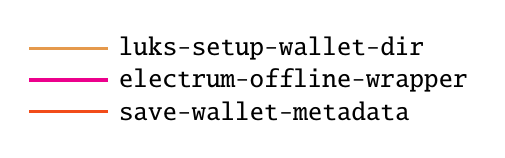
\begin{tikzpicture}
  \draw[orange,very thick]        (0.0,0.8) -- (1.0,0.8) node[at end,right] {\textcolor{black}{\texttt{luks-setup-wallet-dir}}};
  \draw[magenta,very thick]        (0.0,0.4) -- (1.0,0.4) node[at end,right] {\textcolor{black}{\texttt{electrum-offline-wrapper}}};
  \draw[darkorangered,very thick]  (0.0,0.0) -- (1.0,0.0) node[at end,right] {\textcolor{black}{\texttt{save-wallet-metadata}}};
\end{tikzpicture}

\end{document}
